\subsection{Visualizing alignments with \prog{ssu-draw}}

Because SSU rRNA is about 1500 nt, SSU alignments of even a few
sequences are difficult to view in a meaningful way, and this is
especially true if the alignments contain thousands of sequences.
The \prog{ssu-draw} program can be used to generate secondary
structure diagrams for displaying alignment statistics, such as
location and frequency of insertions and deletions, as well as
individual aligned sequences. \prog{ssu-draw} can only be used for
alignments created using the three default models; it cannot
be used for alignments to models created using \prog{ssu-build}.
To draw alignment statistic diagrams of our \prog{myseqs} example
dataset, do:

\user{ssu-draw myseqs}

Two new files will be created for each of the alignments, as reported
to the screen:

\begin{sreoutput}
# Drawing secondary structure diagrams...
#
# alignment file name  structure diagram file  # pages  tabular data file      
# -------------------  ----------------------  -------  -----------------------
  myseqs.archaea.stk   myseqs.archaea.pdf            9  myseqs.archaea.drawtab 
  myseqs.bacteria.stk  myseqs.bacteria.pdf           9  myseqs.bacteria.drawtab
  myseqs.eukarya.stk   myseqs.eukarya.pdf            9  myseqs.eukarya.drawtab 
\end{sreoutput}

The structure diagram files will be PDF format only if you have the
program \prog{ps2pdf} installed and in your PATH, otherwise they will
be postscript files (see the \prog{ssu-draw} manual page for more
information). 

Take a look at the nine page \prog{myseqs.archaea.pdf} or
\prog{myseqs.archaea.ps} file \footnote{For Mac users: postscript
  viewers on the Mac OS are somewhat nonstandard, but Mac OS X's
  Preview application should be able to view either type of file.}
Page 2 of this file is included in this
guide as Figure~\ref{myseqs-archaea-info}. 

Each page shows the same secondary structure template, it is 1508
consensus positions for archaea and includes 471 basepairs as
indicated at the top of each page. Each of the nine pages displays a
different alignment statistic on each of these 1508 consensus
positions. Page 1 shows the alignment consensus sequence which is
defined by the most common nucleotide present in the alignment
\prog{myseq.archaea.stk} at each consensus position. Page 2 shows the
information content per consensus position in a heatmap-like color
scheme; blue positions are highly conserved, red positions are higly
variable. Page 3 shows the mutual information from basepaired nucleotides
as a heatmap. Page 4 and 5 show the frequency and average length of
insertions that occur after each consensus position. An inserted nucleotide
is one that does not align to a consensus position. Importantly, these
nucleotides are not aligned by \prog{ssu-align} but rather simply
inserted between the two appropriate consensus columns. Pages 6 
shows the frequency of all deletions (gaps) in the alignment. Page 7
shows the frequecy of 'internal' deletions, these are deletions that
occur after the first nucleotide and before the final nucleotide in
their corresponding sequence. Page 8 shows the average posterior
probability (confidence estimate) per consensus position. Finally,
page 9 shows the fraction of sequences that span each position,
i.e. that have a nongap nucleotide occuring at or before the
position and a nongap nucleotide occuring at or after the
position. 

You may have noticed that while the majority of positions are drawn as
square cells, some of the positions are open circles. These are the
positions that are excluded by the mask we created earlier using the
command \prog{ssu-mask myseqs} (not the command with
\prog{-d}). As it has done in this case, \prog{ssu-draw} will
automatically use masks to show excluded positions on the diagrams if
\prog{ssu-mask} has already been used on this directory. To use the
default masks discussed in the masking section of this tutorial, use 
the \prog{-d} option (\prog{ssu-mask -d myseqs}), but note that this
will overwrite the files we've just created above unless you also use
the \prog{--key-out} option (e.g. \prog{ssu-mask --key-out df -d
  myseqs}) as shown previously in the masking section.

By default, alignment summary diagrams are drawn as solid
color cells per position, but the consensus sequence can be overlaid
on the colored cells using the \prog{--cnt} option to \prog{ssu-draw}.

The \prog{.drawtab} suffixed files include tabular delimited data
corresponding to the statistics shown in the structure diagrams. In
these files, lines that start with \prog{\#} are comment lines, are
not tabular, and are meant to explain each tab-delimited field. The
comments also explain how the statistics, such as information content
and mutual information, are calculated.

\begin{figure}
  \begin{center}
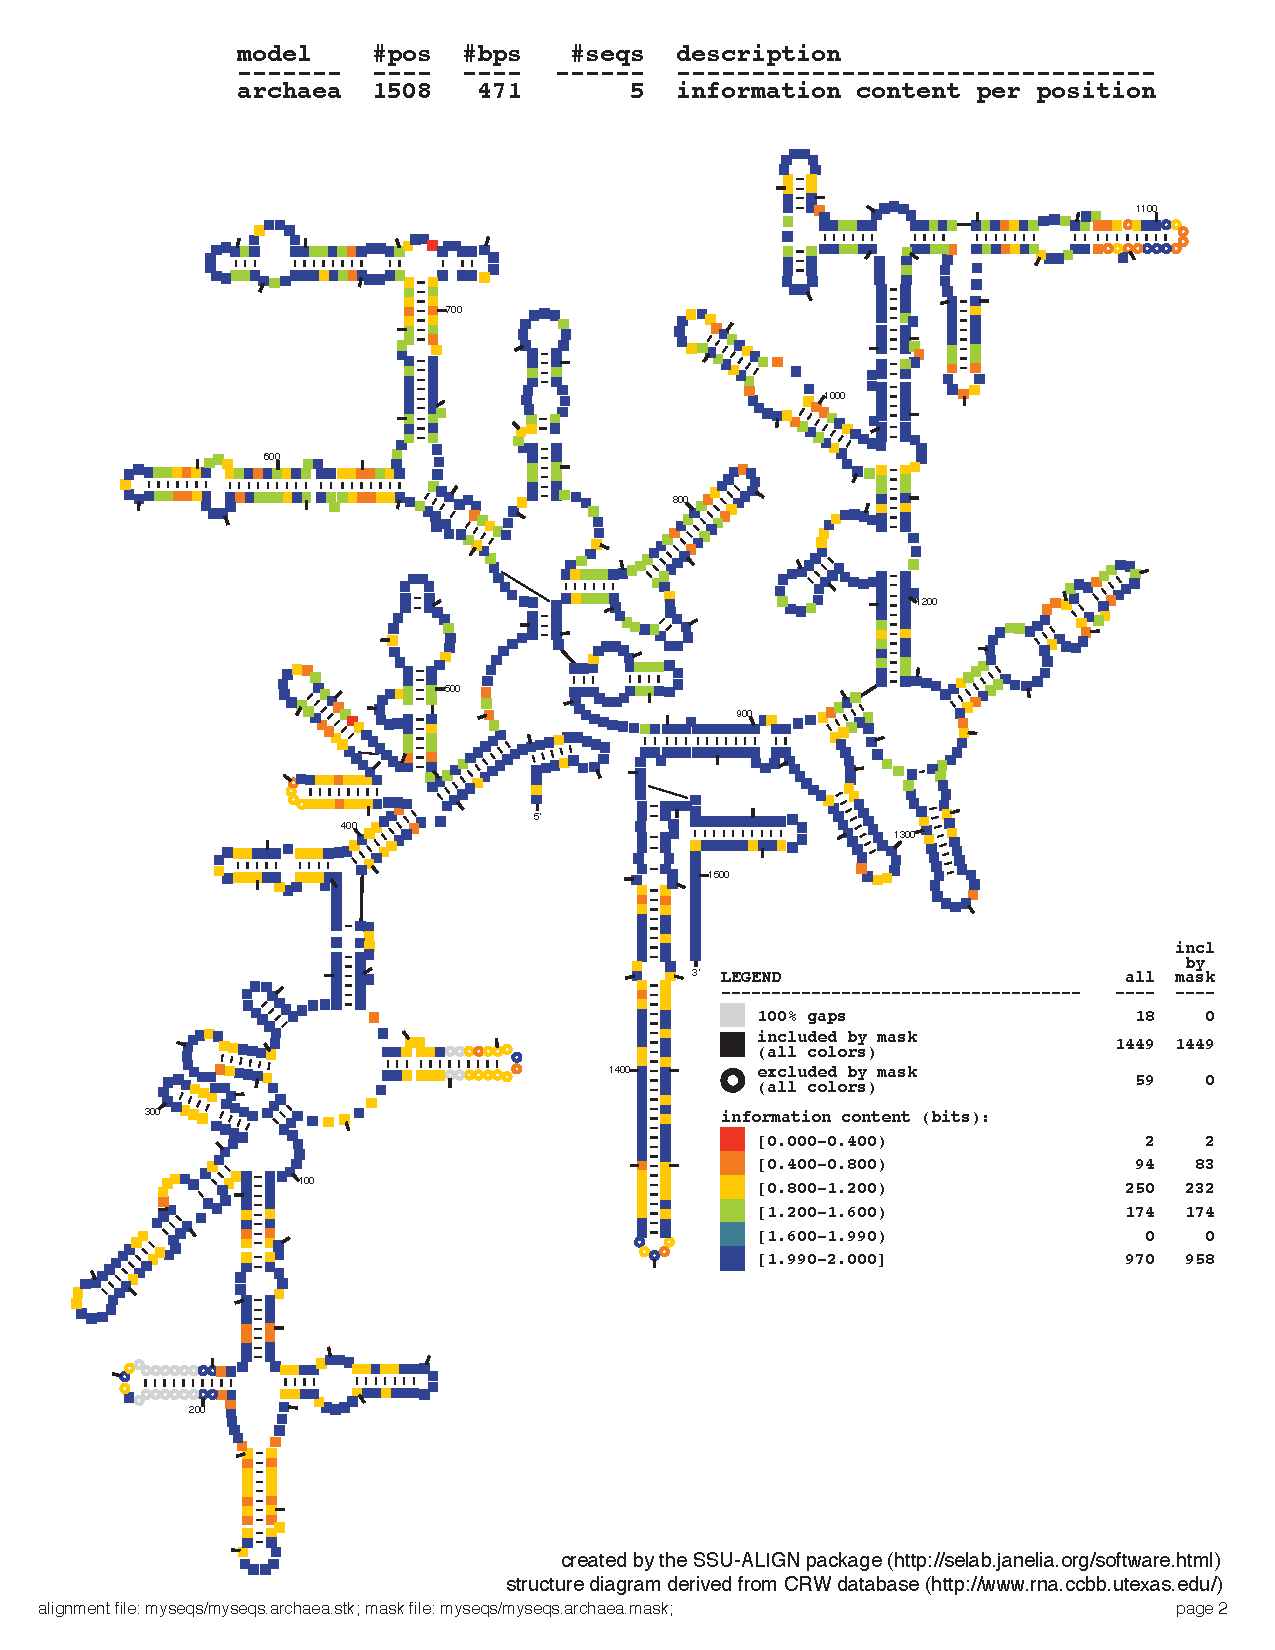
\includegraphics[width=6.5in]{Figures/myseqs-archaea-info}
        \caption[Information content per consensus position of the
          archaeal alignment created in the tutorial].
  \end{center}
\label{fig:myseqs-archaea-info}
\end{figure}

\subsubsection{Drawing individual aligned sequences}

In addition to drawing alignment summary diagrams, \prog{ssu-draw} can
be used to create secondary structure diagrams of individual aligned
SSU sequences using the \prog{--indi-all} option:

\user{ssu-draw --indi-all myseqs}

As before, this command will create the nine-page alignment summary
diagram files, but it will also create \prog{indiall.pdf} suffixed
files which display each sequence in the alignment. 

Take a look at {myseqs.archaea.indiall.pdf} or
{myseqs.archaea.indiall.ps}. This file has 10 pages, two per
sequence. Pages 7 and 8 which display a Thermococcus sequence are
included as Figures~\ref{fig:myseqs-archaea-indi-1} and
\ref{fig:myseqs-archaea-indi-2}.

The first page for each sequence is the aligned sequence with
nucleotides colored by basepair type, and background cells colored by
number of inserts after each nucleotide (blank (white) backgrounds
predominate, indicating 0 inserted nts after those
positions). Additionally, nucleotides that differ from the most
frequent nucleotide at each position are outlined, with thicker
outlines indicating the most frequent nucleotide at the position
occurs in more than 75\% of the aligned sequences.

The second page for each sequence occurs immediately after
the first, and displays the posterior probability of each position
using a heatmap scheme: blue positions have high posterior
probability meaning the program is confident these positions are
correctly aligned, while red indicates low confidence and high
ambiguity. 

Be warned that these files can grow very large for large alignments,
especially if they are being created as postscript
files \footnote{When \prog{ssu-draw} creates PDF files it first
  creates postscript files, then converts them to PDF with
  \prog{ps2pdf}, and finally removes the postscript files.}. In
general, the files will be about 1 Mb per 20 sequences for PDFs and 1
Mb per 2 sequences for postscripts. By default, \prog{ssu-draw} will
exit with an error if the output postscript file you're requesting
would exceed 100 Mb in size, to override this warning and create the
file anyway, use the \prog{-f} option.

Instead of drawing all the sequences in the alignment you can pick and
choose which sequences to draw using the \prog{--indi-list}
option. The names of the sequences must be written to a list file,
which simply places each desired sequence names on a separate
line \prog{It might be helpful to use \prog{ssu-mask --list myseqs} to
create lists of all the sequences in each alignment, and then remove
those you don't want.}. An example list of 2 bacterial sequences from
the myseqs dataset is in \prog{tutorial/mytwobac.list}. To draw just
these two sequences, you would execute: 
\prog{ssu-draw -a --indi-list mytwobac.list myseqs/myseqs.bacteria.stk} .
Notice that the \prog{-a} option was also used and instead of using
\prog{myseqs} as the command-line argument we specified the bacterial
alignment. The \prog{-a} option tells \prog{ssu-draw} that the
command-line argument is an alignment file, not a
\prog{ssu-align}-created directory, and it is required for
\prog{--indi-list} to work. 

There are several other options that can be supplied to
\prog{ssu-draw}. See the \prog{ssu-draw} manual page in
section~\ref{sec:manpages} for more information. 

\begin{figure}
  \begin{center}
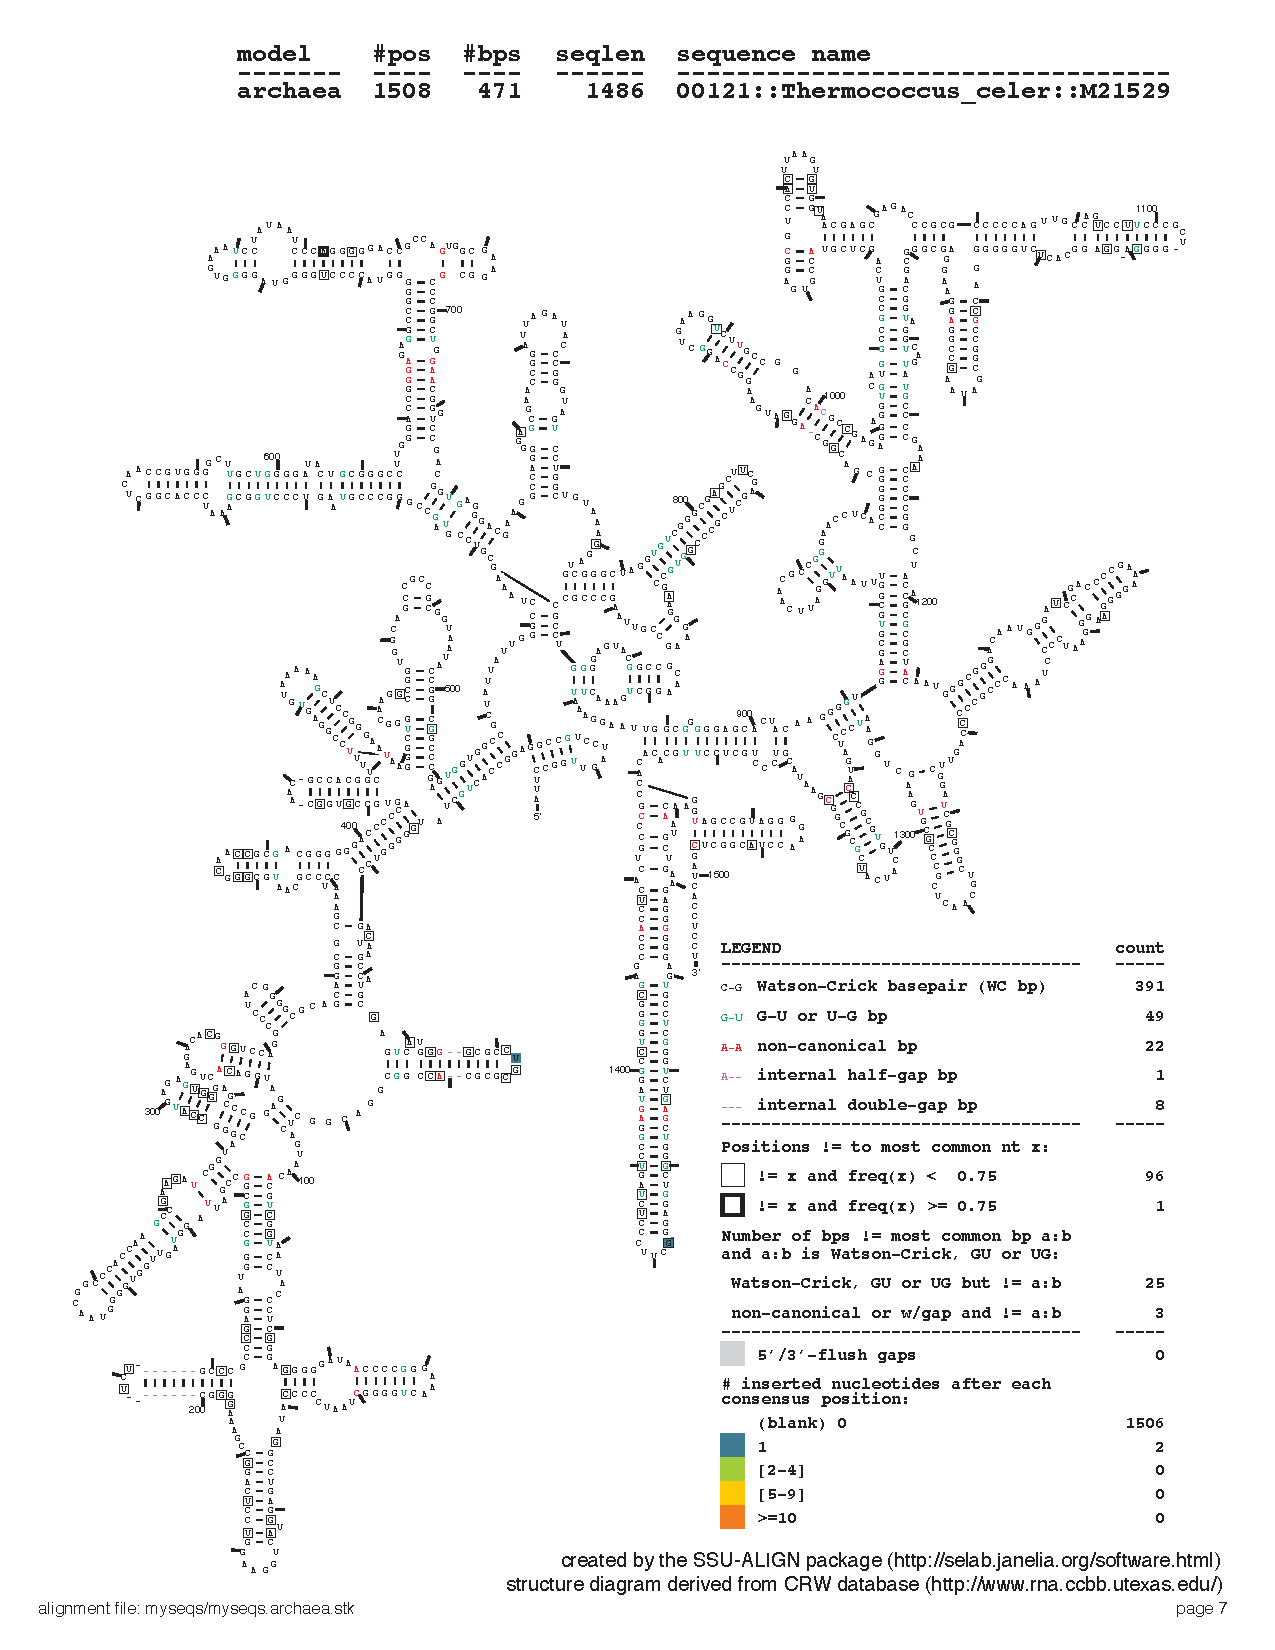
\includegraphics[width=6.5in]{Figures/myseqs-archaea-indi-1}
        \caption[Information content per consensus position of the
          archaeal alignment created in the tutorial].
  \end{center}
\label{fig:myseqs-archaea-indi-1}
\end{figure}

\begin{figure}
  \begin{center}
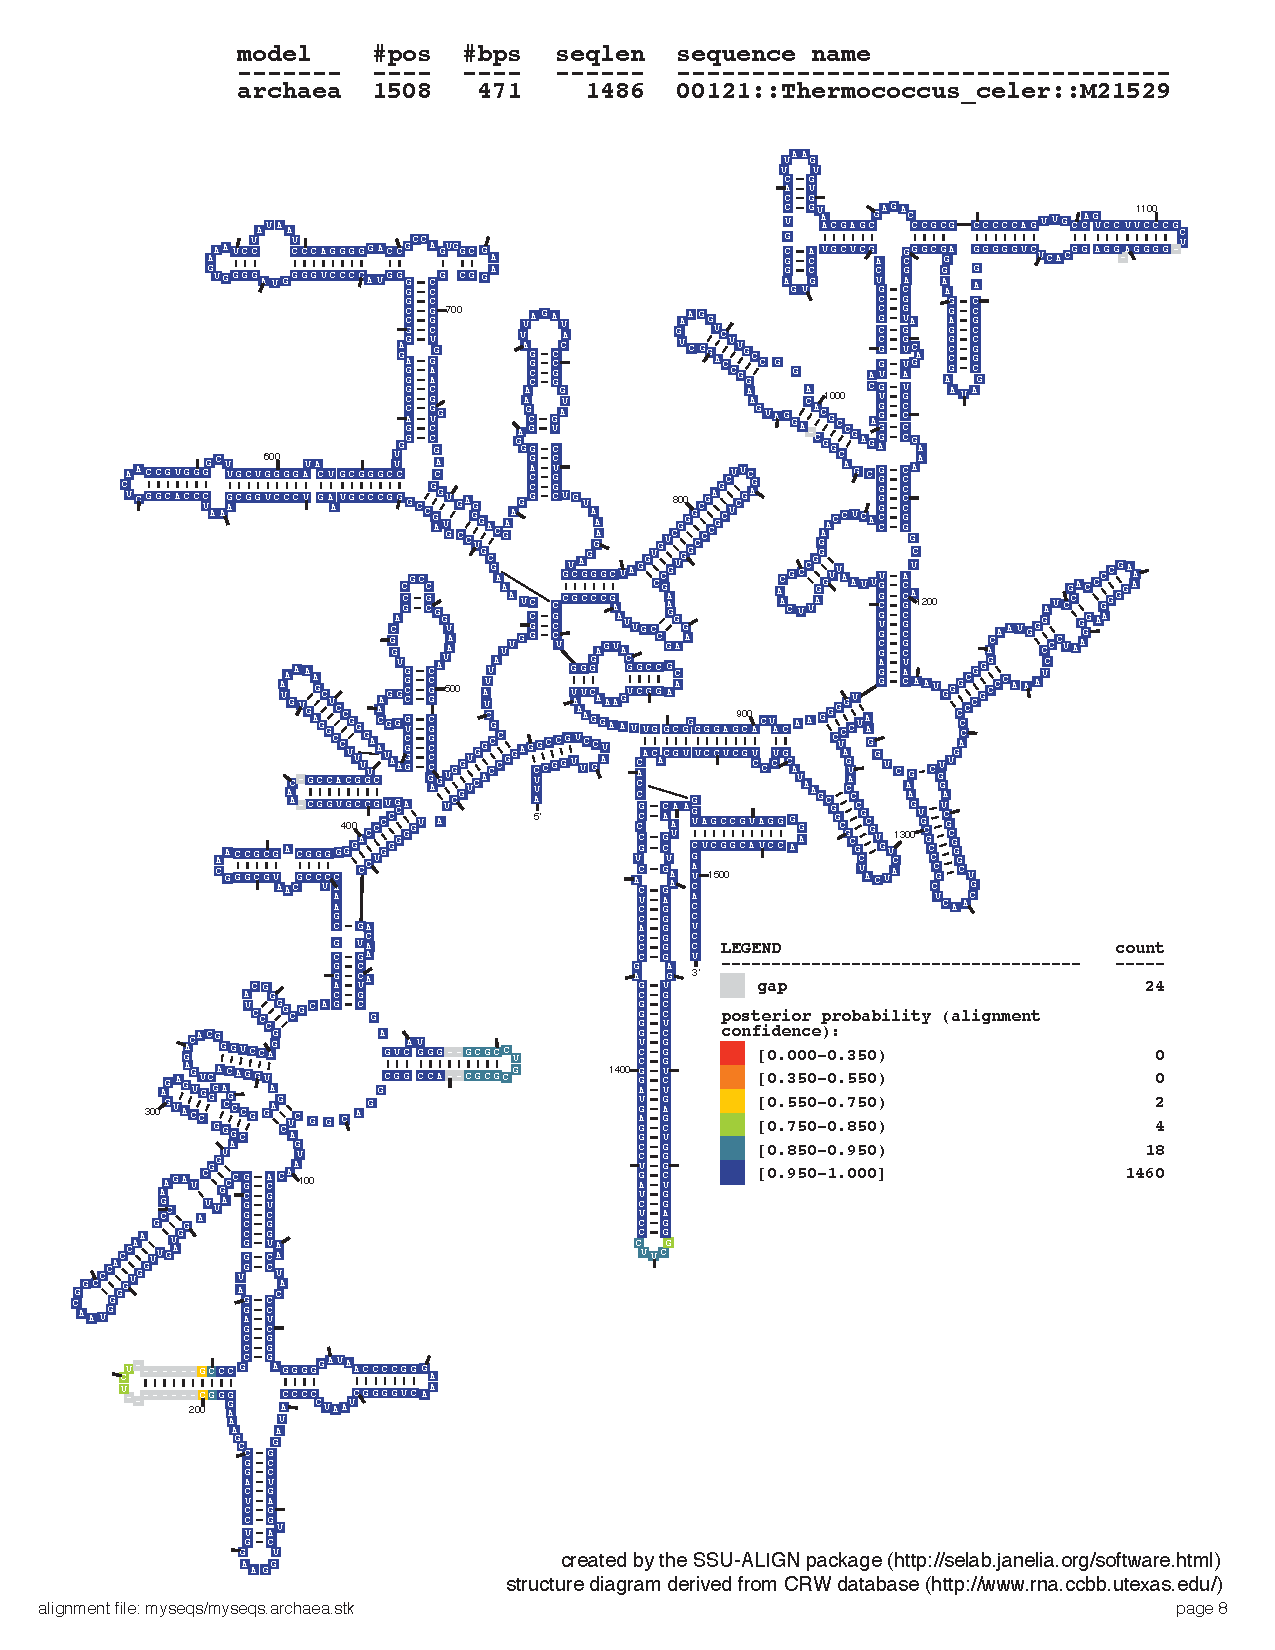
\includegraphics[width=6.5in]{Figures/myseqs-archaea-indi-2}
\caption[Information content per consensus position of the
  archaeal alignment created in the tutorial]. \textbf{Information content per consensus position of the
  archaeal alignment created in the tutorial}.
  \end{center}
\label{fig:myseqs-archaea-indi-2}
\end{figure}
